\documentclass[../Head/Main.tex]{subfiles}
\begin{document}

\subsubsection{Marble detection}
\label{subsubsec:Implementation_marble}
The marble detection method \texttt{find\_marbles()} processes the datapoints by checking if a point satisfies either one of the marble conditions. If so, it breaks and calculates the parameters described in section \ref{subsec:DesignMarbleDetection}.\par 
One marble condition is a threshold for the range between two point and is defined to 0.2. This condition ensures that a marble can be detected from points from a partial circle periphery. Another marble condition is a range, that ensures that a marble can be detected in outer edges of the sensor range. This range is defined as the subtraction of marble condition one from the sensor range for the LIDAR sensor.

\clearpage
To test the performance and robustness of the algorithm a  test with several repetitions were conducted. This test in described in appendix (\ref{test:MarbleDetection}).

\begin{figure}[H]
  \begin{subfigure}[b]{0.3\textwidth}
  	\centering
    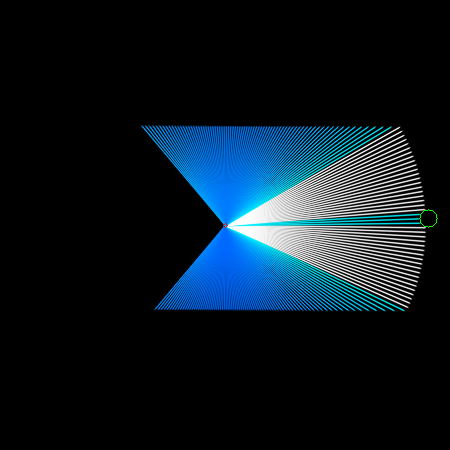
\includegraphics[width=0.9\textwidth]{Lidar/Test_2_marbles}
    \caption{Illustration of data for test 2}
    \label{fig:MarbleTest2}
  \end{subfigure}
  \hfill
  \begin{subfigure}[b]{0.3\textwidth}
  	\centering
    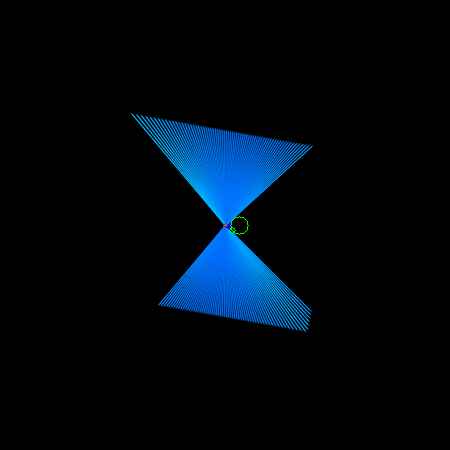
\includegraphics[width=0.9\textwidth]{Lidar/Test_3_marbles}
    \caption{Illustration of data for test 3}
    \label{fig:MarbleTest3}
  \end{subfigure}
  \hfill
  \begin{subfigure}[b]{0.3\textwidth}
    \centering
    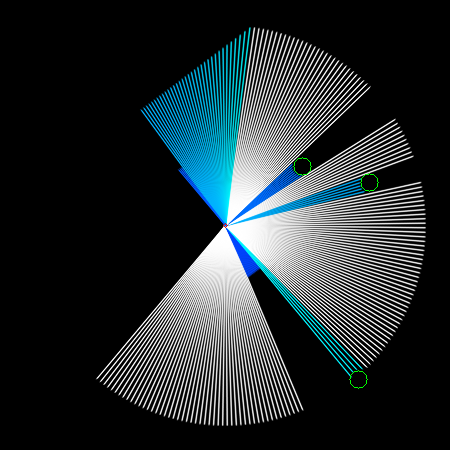
\includegraphics[width=0.9\textwidth]{Lidar/Test_5_marbles}
    \caption{Illustration of data for test 5}
    \label{fig:MarbleTest5}
  \end{subfigure}
  \caption{Illustration of data for marble detection tests}
\end{figure}
The marble detected in figure (\ref{fig:MarbleTest2}) verifies that the marble condition holds, and that a marble can be detected in the outer edge of the detection area. The same applies for one of the marbles on figure (\ref{fig:MarbleTest5}). Figure (\ref{fig:MarbleTest5}) also shows that marbles can be detected anywhere in the sensor range. Sometimes the marble detection algorithm can detect an extra marble, where there is only one, as shown on figure (\ref{fig:MarbleTest3}). 
\begin{figure}[H]
  \begin{subfigure}[b]{0.5\textwidth}
  	\centering
    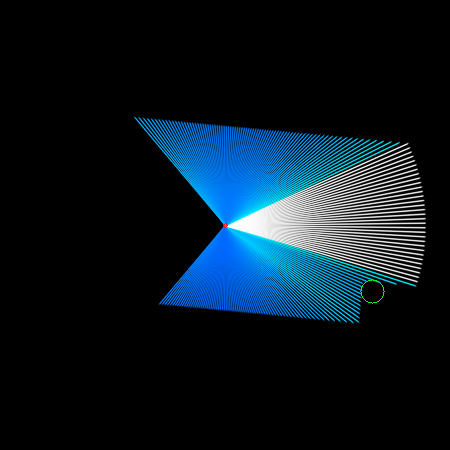
\includegraphics[width=0.54\textwidth]{Lidar/Test_6_marbles}
    \caption{Illustration of data for test 6}
    \label{fig:MarbleTest6}
  \end{subfigure}
  \hfill
  \begin{subfigure}[b]{0.5\textwidth}
  	\centering
    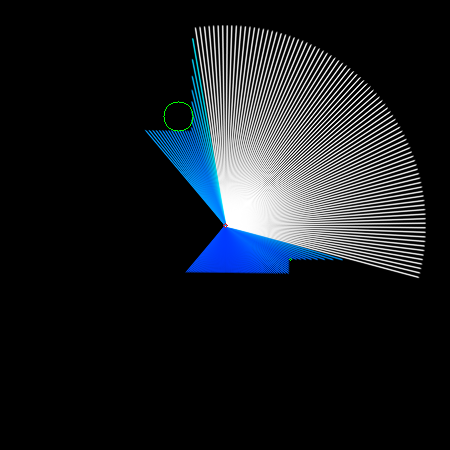
\includegraphics[width=0.54\textwidth]{Lidar/Test_7_marbles}
    \caption{Illustration of data for test 7}
    \label{fig:MarbleTest7}
  \end{subfigure}
  \caption{Illustration of data for marble detection tests}
\end{figure}
Figure (\ref{fig:MarbleTest6}) and (\ref{fig:MarbleTest7}) indicates that a marble can be detected in a corner, which might as well give problems. Due to the fact, that the robot will steer against marbles in the corners, the robot will hit an obstacle and tilt.\par
Due to this, the marble detection algorithm is not robust and do not have a good performance, since it only gives the expected outcome in some cases and in most cases detects marbles, where there is none.

\end{document}